\documentclass{beamer}
\usetheme{Warsaw}

\usepackage[utf8]{inputenc}
\usepackage{fancybox}
\usepackage{multimedia} 
\usepackage{subfig}
\usepackage{amsmath}
\usepackage{hyperref}
\usepackage[all]{xy}
\usepackage{algorithm}
%\usepackage{arevmath}     % For math symbols
\usepackage[noend]{algpseudocode}

\begin{document}


\title[Angewandte Mathematik] % (optional, only for long titles)
{Angewandte Mathematik
\\
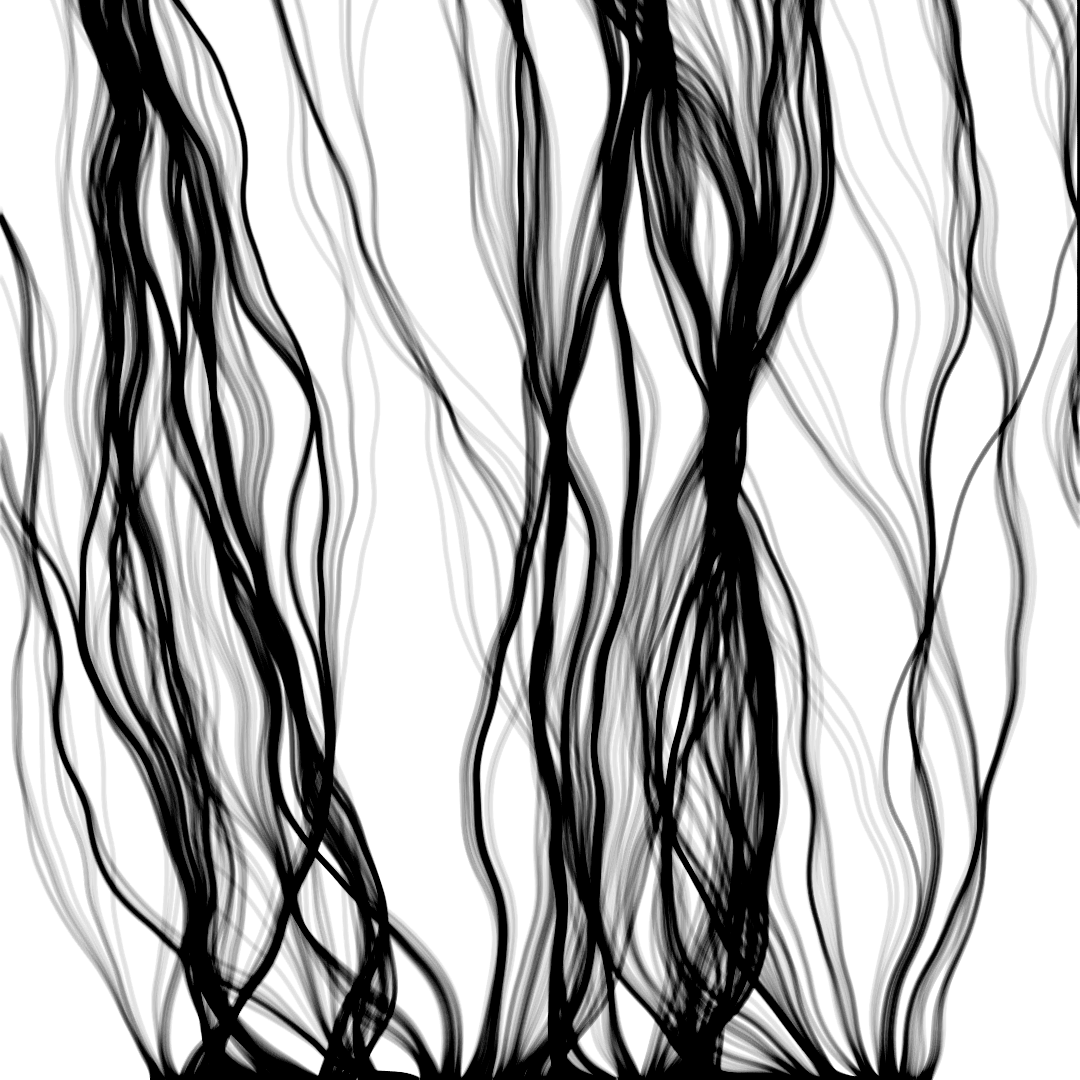
\includegraphics[scale=0.15]{images/cover}
}
\subtitle{}
\author[Dr. Johannes Riesterer] % (optional, for multiple authors)
{Dr.  rer. nat. Johannes Riesterer}

\date[KPT 2004] % (optional)
{}

\subject{Angewandte Mathematik}




\begin{frame}
    \frametitle{Angewandte Mathematik}
\framesubtitle{Dynamische Systeme }
\begin{block}{Motivation}
Gegeben ist ein zeitabhängiges System $t \mapsto x(t)$. 
Möchten verstehen, wie sich $x(t)$ über die Zeit entwickelt. 
Zu festen Zeitpunkten $t_0, \cdots t_n $ lässt sich $x(t_i)$ messen und damit $x'(t_i) \cong \frac{x(x(t_i) - x(t_{i-1}))}{t_i - t_{i-1}}$ näherungsweise bestimmen. Im allgemeinen ist die Ableitung $x'(t) = f(x(t), t)$ eine Funktion in der Zeit und der Funktion selbst. 
\end{block}
 \end{frame}

\begin{frame}
    \frametitle{Angewandte Mathematik}
\framesubtitle{Dynamische Systeme }
\begin{block}{Beispiel}
$(1) \;x'(t) = \mu x(t)$.  
Dann ist $x(t)= c e^{\mu t}$ für alle $c \in \mathbb{R}$ eine Lösung. Ist $x(0) = x_0$, so ist   $x(t)= x_0 e^{\mu t}$ eine Lösung von (1) mit $x(0) = x_0$. 
\end{block}
 \end{frame}

\begin{frame}
    \frametitle{Angewandte Mathematik}
\framesubtitle{Dynamische Systeme }
\begin{block}{System von Differentialgleichungen}
Ein System von Differentialgleichungen $1$-ter Ordnung ist ein System von Gleichungen
\begin{align*}
\begin{matrix} x_1'(t) = f_1(t, x_1, \cdots, x_n ) \\  \\ x_2'(t) = f_2(t, x_1, \cdots, x_n ) \\  \vdots \\  x_n'(t) = f_n(t, x_1, \cdots, x_n )\end{matrix}
\end{align*}
Werden zusätzlich die Anfanfsbedingungen $x_1(t_0)= x_0^1, \dots ,  x_n(t_0) = x_0^n$ vorgegebenen, so spricht man von einem Anfangswertproblem.
Eine Lösung ist eine Funktion $x : I \subset \mathbb{R} \to \mathbb{R}^n$, deren Koordinatenfunktionen diese Bedingungen erfüllt.
\end{block}
 \end{frame}

\begin{frame}
    \frametitle{Angewandte Mathematik}
\framesubtitle{Dynamische Systeme }
\begin{block}{System von Differentialgleichungen}

Ein Anfangswertproblem $n$-ter Ordnung
 $$ x^{(n)}(t) = f(t, x^{(n)}, x^{(n-1)} , \cdots , x', x) $$ mit  $x(t_0) = x_0 ; x'(t_0) = x_1; \cdots ; x^{n-1}(t_{0})= x_{n-1}  $ ist äquivalent zu dem System von   Differentialgleichungen $1$-ter Ordnung
\begin{align*}
\begin{matrix} x_1'(t) = x_2(t) \\  \\ x_2'(t) = x_3(t) \\  \vdots  \\ x_n'(t) = f(t, x_1, \cdots, x_n )\end{matrix}
\end{align*}
mit den Anfangswertbedingungen  $x_1(t_0) = x_0 , x_2(t_0) = x_1, \cdots , x_{n-1}(t_{0})= x_{n-1} $.
\end{block}


 \end{frame}


\begin{frame}
    \frametitle{Angewandte Mathematik}
\framesubtitle{Dynamische Systeme }
\center
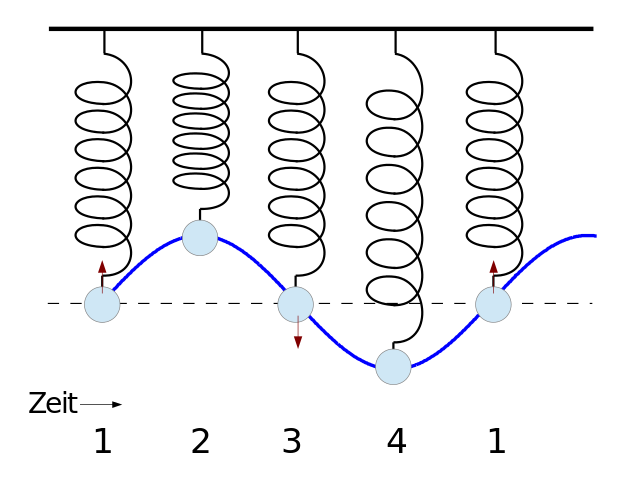
\includegraphics[scale=0.35]{images/federpendel}

 \end{frame}




\begin{frame}
    \frametitle{Angewandte Mathematik}
\framesubtitle{Dynamische Systeme }
\begin{block}{Harmonischer Oszillator}
$x''(t) = -x(t)$.
\end{block}
\begin{block}{Harmonischer Oszillator}
\begin{align*}
    \frac{d}{dt}\begin{pmatrix}
        x_1(t) \\ x_2(t)
    \end{pmatrix} = 
\begin{pmatrix}
    0 & -1  \\ 1 & 0
\end{pmatrix} \cdot
\begin{pmatrix} 
    x_1(t) \\ x_2(t)
\end{pmatrix} 
\end{align*}
\end{block}
 \end{frame}





\begin{frame}
    \frametitle{Angewandte Mathematik}
\framesubtitle{Dynamische Systeme }
\begin{block}{System von Differentialgleichungen}

Für eine  vekorwertige Funktion  $f : I   \to \mathbb{R}^n; f(t) : = \begin{pmatrix} f_1(t)  \\ \vdots \\ f_n(t) \end{pmatrix}$ definieren wir das Integral komponentenweise durch
$$\int_{a}^{b}  f(t) dt := \begin{pmatrix} \int_{a}^{b}  f_1(t) dt  \\ \vdots \\ \int_{a}^{b}  f_n(t) dt \end{pmatrix} \; .$$
\end{block}
 \end{frame}

\begin{frame}
    \frametitle{Angewandte Mathematik}
\framesubtitle{Dynamische Systeme }
\begin{block}{System von Differentialgleichungen}
Ein Weg $\varphi : I \subset \mathbb{R} \to \mathbb{R}^n$ ist genau dann Lösung des AWP $\varphi'(t) = F(t , \varphi)$ mit $ \varphi(t_0)= x_0$, wenn
$$ \varphi(t) =  x_0 + \int_{t_0}^{t} F(t, \varphi) dt$$
gilt.
\end{block}
\begin{block}{Beweis}
Folgt direkt durch komponentenweise Anwendung des Hauptsatzes der Integral- und Differentialrechnung.
\end{block}
 \end{frame}



\begin{frame}
    \frametitle{Angewandte Mathematik}
\framesubtitle{Dynamische Systeme }

\begin{block}{Volterra-Lotka System}
https://de.wikipedia.org/wiki/Lotka-Volterra-Gleichungen
\end{block}
 \end{frame}


\begin{frame}
    \frametitle{Angewandte Mathematik}
\framesubtitle{Dynamische Systeme }
\begin{block}{System von Differentialgleichungen}
Ein Vektorfeld ist eine Abbildung $$v : \Omega \subset \mathbb{R}^n \to \mathbb{R}^n \; ,$$ die jedem Punkt $x  \in \Omega$ einen Vektor $v(x) \in \mathbb{R}^n$ zuordnet.
\end{block}
\begin{figure}[H]
      \centering
    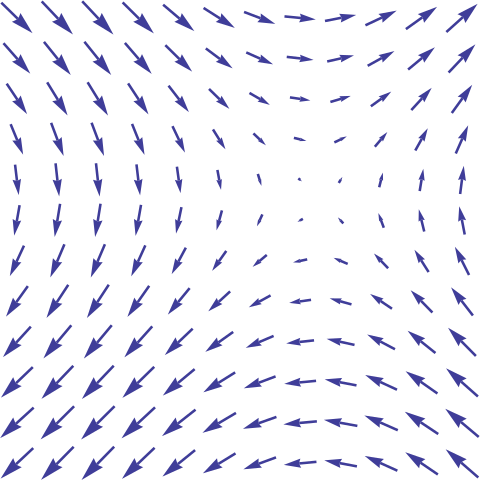
\includegraphics[width=0.3\textwidth]{images/480px-VectorField.png}
\caption{Quelle: Wikipedia:https://en.wikipedia.org/wiki/Vector\_field\#/media/File:VectorField.svg}
\end{figure}

 \end{frame}

\begin{frame}
    \frametitle{Angewandte Mathematik}
\framesubtitle{Dynamische Systeme }
\begin{block}{System von Differentialgleichungen}
Ein Weg $\varphi : I \subset \mathbb{R} \to \mathbb{R}^n$ heißt Integralkurve in dem Vektorfeld $v : \Omega \subset \mathbb{R}^n \to \mathbb{R}^n$, falls 
$$\varphi' (t) = v(\varphi(t))$$ gilt für alle $t \in  I$.
\end{block}
\begin{figure}[H]
      \centering
    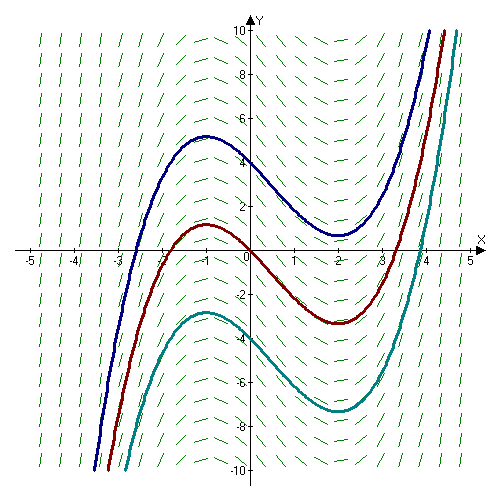
\includegraphics[width=0.3\textwidth]{images/Slope_Field.png}
\caption{Quelle: Wikipedia:https://en.wikipedia.org/wiki/Integral\_curve\#/media/File:Slope\_Field.png}
\end{figure}

 \end{frame}


\begin{frame}
    \frametitle{Angewandte Mathematik}
\framesubtitle{Dynamische Systeme }
\begin{block}{System von Differentialgleichungen}
Ein dynamisches System ist eine  Abbildung $F : U \subset \mathbb{R} \times \mathbb{R}^n \to \mathbb{R}^n$, die jedem Punkt $(t,x)  \in U$ einen Vektor $F(t,x) \in \mathbb{R}^n$ zuordnet. Eine Integralkurve oder Lösung für $F$ ist eine Weg $\varphi : I \to \mathbb{R}^n$ mit 
$$\varphi'(t) = F(t, \varphi(t)) $$
für alles $t \in I$.
\end{block}
 \end{frame}





 \begin{frame}
    \frametitle{Angewandte Mathematik}
\framesubtitle{Dynamische Systeme }
\center
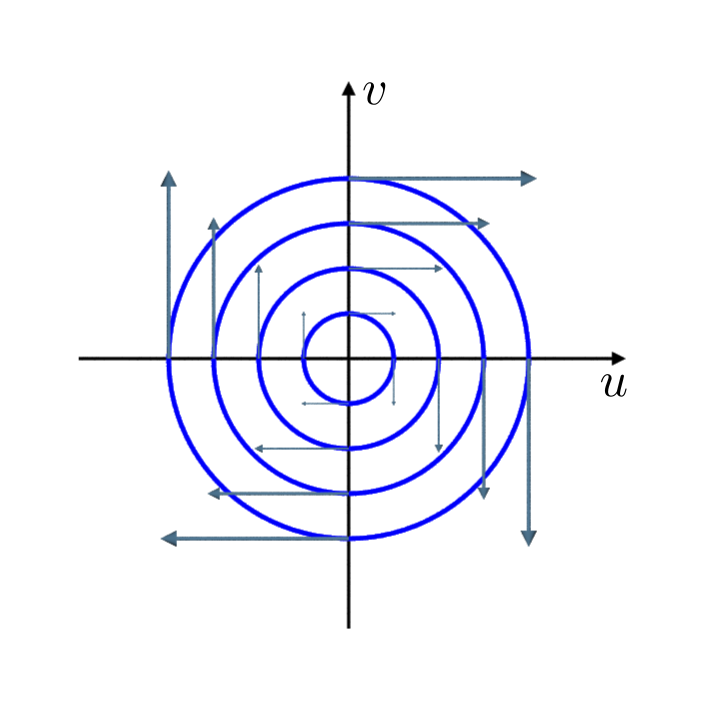
\includegraphics[scale=0.35]{images/harmonicoszillatorphasespace}
 \end{frame}


 \begin{frame}
    \frametitle{Angewandte Mathematik}
\framesubtitle{Dynamische Systeme }

\begin{block}{Lösung Harmonischer Oszillator}
  \begin{align*}
    \frac{d}{dt}\begin{pmatrix}
        x_1(t) \\ x_2(t)
    \end{pmatrix} = 
\begin{pmatrix}
    0 & -1  \\ 1 & 0
\end{pmatrix} \cdot
\begin{pmatrix} 
    x_1(t) \\ x_2(t)
\end{pmatrix} 
\end{align*}

    \begin{align*}
        \begin{pmatrix}
            x_1(t) \\ x_2(t)
        \end{pmatrix} = \begin{pmatrix}
            \cos(t) & -\sin(t)  \\ \sin(t) & \cos(t)
        \end{pmatrix}   \cdot \begin{pmatrix}
            x_1\\ x_2
        \end{pmatrix}
    \end{align*}
\end{block}
 \end{frame}



\begin{frame}
    \frametitle{Angewandte Mathematik}
\framesubtitle{Dynamische Systeme }
\begin{block}{Harmonischer Oszillator}
\begin{align*}
    \frac{d}{dt}\begin{pmatrix}
        x_1(t) \\ x_2(t)
    \end{pmatrix} = 
\begin{pmatrix}
    0 & -1  \\ 1 & 0
\end{pmatrix} \cdot
\begin{pmatrix} 
    x_1(t) \\ x_2(t)
\end{pmatrix} 
\end{align*}
\end{block}

\begin{block}{Lösung Harmonischer Oszillator}
    Anfangswert $\begin{pmatrix}
        x_1 \\ x_2\end{pmatrix} = \begin{pmatrix}
            x_1(t_0) \\ x_2(t_0)\end{pmatrix}$
    \begin{align*}
        \begin{pmatrix}
            x_1(t) \\ x_2(t)
        \end{pmatrix} = e^{ \begin{pmatrix}
            0 & -1  \\ 1 & 0
        \end{pmatrix} t } \cdot \begin{pmatrix}
            x_1\\ x_2
        \end{pmatrix}
    \end{align*}
\end{block}

 \end{frame}


 \begin{frame}
    \frametitle{Angewandte Mathematik}
\framesubtitle{Dynamische Systeme }
\begin{block}{Harmonischer Oszillator}

\begin{align*}
 e^{ \begin{pmatrix}
        0 & -1  \\ 1 & 0
    \end{pmatrix} t } = \sum_{k= 0}^{\infty} \begin{pmatrix}
    0 & -1  \\ 1 & 0
\end{pmatrix}^{k} \frac{t^k}{k!} 
\end{align*}

\end{block}
 \end{frame}


 \begin{frame}
    \frametitle{Angewandte Mathematik}
\framesubtitle{Dynamische Systeme }
\begin{block}{Harmonischer Oszillator}

\begin{align*}
\begin{pmatrix}
        0 & -1  \\ 1 & 0
    \end{pmatrix}^{k}  = \begin{cases} 
        \begin{pmatrix}
            1 & 0  \\ 0 & 1
        \end{pmatrix}; k = 0 \mod 4 \\
        \begin{pmatrix}
            0 & -1  \\ 1 & 0
        \end{pmatrix}; k = 1 \mod 4 \\
        \begin{pmatrix}
            -1 & 0  \\ 0 & -1
        \end{pmatrix}; k = 2 \mod 4 \\
        \begin{pmatrix}
            0 & 1  \\ -1 & 0
        \end{pmatrix}; k = 3 \mod 4
    \end{cases}
\end{align*}
\end{block}
 \end{frame}

 \begin{frame}
    \frametitle{Angewandte Mathematik}
\framesubtitle{Dynamische Systeme }
\begin{block}{Harmonischer Oszillator}

\begin{align*}
\sum_{k= 0}^{n} \begin{pmatrix}
    0 & -1  \\ 1 & 0
\end{pmatrix}^{k} \frac{t^k}{k!} & =
\begin{pmatrix}
    1-\frac{t^2}{2!} + \frac{t^4}{4!}-\frac{t^6}{6!} \cdots & -t +\frac{t^3}{3!} - \frac{t^5}{5!} +\frac{t^7}{7!} \cdots  \\ 1 & 0 \\
    t -\frac{t^3}{3!} + \frac{t^5}{5!} -\frac{t^7}{7!} \cdots  & 1-\frac{t^2}{2!} + \frac{t^4}{4!}-\frac{t^6}{6!}  \cdots
\end{pmatrix} \\
&= \begin{pmatrix}
    \cos(t) & -\sin(t)  \\ \sin(t) & \cos(t)
\end{pmatrix}
\end{align*}
\href{https://de.wikipedia.org/wiki/Taylorreihe}{Link:Trigonometrische Taylorreihen}
\end{block}
 \end{frame}







 \begin{frame}
    \frametitle{Angewandte Mathematik}
\framesubtitle{Dynamische Systeme }

\begin{block}{Harmonischer Oszillator Eigenwerte}
    \begin{align*}
    \det (\begin{pmatrix}
        0 & -1  \\ 1 & 0
    \end{pmatrix} - \lambda E) = 
    \det \begin{pmatrix}
        -\lambda & -1  \\ 1 & -\lambda  
    \end{pmatrix} = \lambda^2 +1 \Rightarrow \lambda_{1,2} = \pm i
\end{align*}
Komplexer Eigenwert.
 \end{block}
 \end{frame}




\begin{frame}
    \frametitle{Angewandte Mathematik}
\framesubtitle{Dynamische Systeme }
\begin{block}{Gedämpftes Pendel}
$\theta''(t) = -L \theta - \underbrace{\mu \theta'}_{\text{drag}}$. $L \theta = mg \sin(\theta)$ 
\end{block}
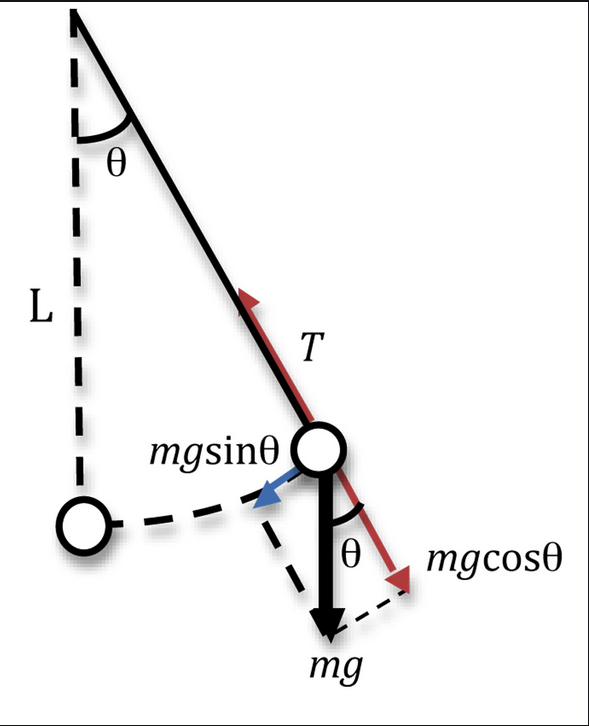
\includegraphics[scale=0.2]{images/pendulum0}
\begin{block}{System gedämpftes Pendel}
    $ \frac{d}{dt}\begin{pmatrix}
        x_1(t) \\ x_2(t)
    \end{pmatrix} = 
    \begin{pmatrix}
        x_2(t) \\ -\mu x_2(t) - \frac{m g}{L} \sin(x_1(t))  
    \end{pmatrix} $ (nicht linear!)
    \end{block}
 \end{frame}

 \begin{frame}
    \begin{block}{Phasenbild gedämpftes Pendel}
    $\mu = 0$
    \frametitle{Angewandte Mathematik}
\framesubtitle{Dynamische Systeme }
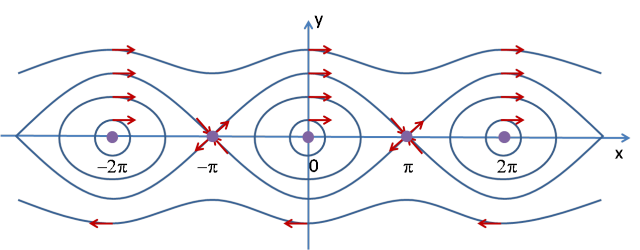
\includegraphics[scale=0.9]{images/pendulum1}
    \end{block}
\end{frame}







 \begin{frame}
\framesubtitle{Numerische Lösungen}
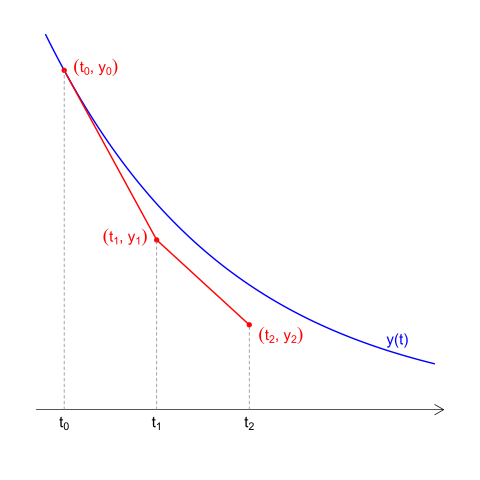
\includegraphics[scale=0.6]{images/euler}

\end{frame}




 \begin{frame}
\framesubtitle{Numerische Lösungen}
    \begin{block}{Euler Verfahren}

$\dot{y}=f(t,y), \quad  y(t_0)=y_0$
\begin{align}
t_k=t_0+kh \\
y_{k+1}=y_k+hf(t_k,y_k)
\end{align}

    \end{block}
\end{frame}






 \begin{frame}
\framesubtitle{Numerische Lösungen}
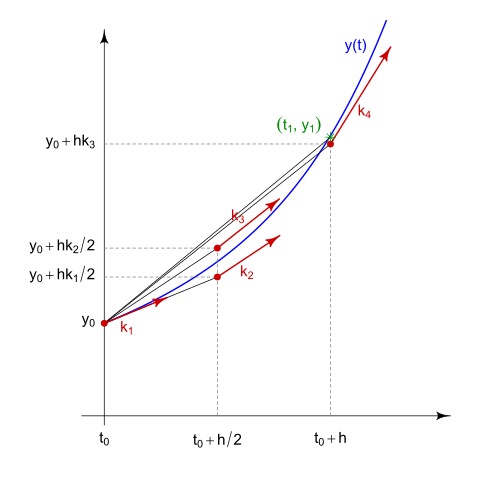
\includegraphics[scale=0.6]{images/Runge-Kutta}

\end{frame}

 \begin{frame}
\framesubtitle{Numerische Lösungen}
    \begin{block}{Runge Kuta Verfahren}
$\dot{y}=f(t,y), \quad  y(t_0)=y_0$
\begin{align}
y_{n+1} &= y_n + \frac{h}{6}\left(k_1 + 2k_2 + 2k_3 + k_4 \right),\\
t_{n+1} &= t_n + h \\
 k_1 &= \ f(t_n, y_n), \\
 k_2 &= \ f\!\left(t_n + \frac{h}{2}, y_n + h \frac{k_1}{2}\right), \\ 
 k_3 &= \ f\!\left(t_n + \frac{h}{2}, y_n + h \frac{k_2}{2}\right), \\
 k_4 &= \ f\!\left(t_n + h, y_n + h k_3\right).
\end{align}
    \end{block}
\end{frame}



\end{document}